\documentclass[aspectratio=1610]{beamer}
\setbeamersize{text margin left=7mm,text margin right=5mm}
\usefonttheme[onlymath]{serif}
\usetheme{default}
\usefonttheme{professionalfonts}
%\setbeamertemplate{navigation symbols}{} 
\beamertemplatenavigationsymbolsempty
\addtobeamertemplate{navigation symbols}{}{
    \usebeamerfont{footline}
    \usebeamercolor[fg]{footline}
    %\hspace{1em}
    \footnotesize\insertframenumber\,%/\inserttotalframenumber
}

% cSpell:disable
\definecolor{rcomment}{rgb}{0.3, 0.3, 0.3}  % darkgrey
\definecolor{rred}{rgb}{0.7,0.2,0.2}        % red
\definecolor{rblue}{rgb}{0.2,0.2,0.7}       % blue (blended blue of beamer)
\definecolor{rpurple}{rgb}{0.45, 0.0, 0.9}  % violett
\definecolor{rpink}{rgb}{0.8, 0.0, 0.4}     % pink
\definecolor{rgreen}{rgb}{0.1, 0.5, 0.1}    % darkgreen
\definecolor{rorange}{rgb}{0.8, 0.4,0}      % orange
\definecolor{rblack}{rgb}{0, 0, 0}          % black
\definecolor{deeptuerkis}{rgb}{0, 0.5, 0.5} % Türkis
\definecolor{darkgreen}{rgb}{0,0.5,0}
\definecolor{blendedblue}{rgb}{0.2,0.2,0.7}
\newcommand{\important}[1]{{\color{green!60!black}#1}}

% \documentclass{beamer}
% \mode<presentation> {
%   \usetheme{Singapore}
%   \setbeamertemplate{navigation symbols}{}
%   \setbeamertemplate{footline}[frame number]
% }

\usepackage[utf8]{inputenc}
\usepackage{caption}
\usepackage{nicefrac}
\usepackage{varwidth}
\usepackage{amsmath}
\usepackage{hyperref}
\usepackage{color}
\usepackage{xcolor}
\usepackage{appendixnumberbeamer}
\usepackage{booktabs}
\usepackage{multirow}
\usepackage{siunitx}	% Allows to format numbers in tables
\usepackage{makecell}	% Allows line breaks in table text
\usepackage{multirow}	% Allows line breaks in table text
\usepackage{graphicx}
% \usepackage[table,xcdraw]{xcolor}
% Beamer presentation requires \usepackage{colortbl} instead of \usepackage[table,xcdraw]{xcolor}
\usepackage{colortbl}

\usepackage{pgfplots}
\pgfplotsset{compat=newest}
\usepgfplotslibrary{statistics}

\usepackage{tikz}
\usetikzlibrary{arrows,automata}
\usetikzlibrary{datavisualization}
\usetikzlibrary{positioning}
\usetikzlibrary{calc}
\usetikzlibrary{patterns}
\usetikzlibrary{matrix}
\usetikzlibrary{decorations.pathreplacing}
\usetikzlibrary{shapes.geometric, arrows, arrows.meta}

\tikzstyle{vertex} = [circle, draw=black, fill=black, minimum width=0.15cm, inner sep=0cm, text centered]
\tikzstyle{arc} = [thick,->,>=stealth]
\tikzstyle{emphvertex} = [circle, draw=red, fill=red, minimum width=0.15cm, inner sep=0cm, text centered]
\tikzstyle{empharc} = [thick,->,>=stealth, draw=red]
\tikzstyle{vertex-green} = [circle, draw=ForestGreen, fill=ForestGreen, minimum width=0.15cm, inner sep=0cm, text centered]
\tikzstyle{arc-green} = [very thick,->,>=stealth, draw=ForestGreen] %thick, very thick, ultra thick
\tikzstyle{bgvertex} = [circle, draw=black!40, fill=black!40, minimum width=0.15cm, inner sep=0cm, text centered]
\tikzstyle{bgarc} = [draw=black!40,thick,->,>=stealth]
\tikzstyle{move} = [thick, ->, -Implies, double,double distance=0.7mm]
\tikzstyle{cyclearc} = [thick,->,>=stealth,draw=red]
\tikzstyle{gets} = [thick, ->, -{Implies[length=5mm, width=3mm]}, double, double distance=1mm]

\usepackage{rotating}
\usepackage{subcaption}
\usepackage{cancel}

\newcommand\hcancel[2][black]{\setbox0=\hbox{$#2$}%
\rlap{\raisebox{.45\ht0}{\textcolor{#1}{\rule{\wd0}{1pt}}}}#2} 


% CHEATING DASH FROM https://tex.stackexchange.com/a/133357/128068
\tikzset{
	cheating dash/.code args={on #1 off #2}{
		% Use csname so catcode of @ doesn't have do be changed.
		\csname tikz@addoption\endcsname{%
			\pgfgetpath\currentpath%
			\pgfprocessround{\currentpath}{\currentpath}%
			\csname pgf@decorate@parsesoftpath\endcsname{\currentpath}{\currentpath}%
			\pgfmathparse{\csname pgf@decorate@totalpathlength\endcsname-#1}\let\rest=\pgfmathresult%
			\pgfmathparse{#1+#2}\let\onoff=\pgfmathresult%
			\pgfmathparse{max(floor(\rest/\onoff), 1)}\let\nfullonoff=\pgfmathresult%
			\pgfmathparse{max((\rest-\onoff*\nfullonoff)/\nfullonoff+#2, #2)}\let\offexpand=\pgfmathresult%
			\pgfsetdash{{#1}{\offexpand}}{0pt}}%
	}
}

\usepackage{mathtools}
%\usepackage{algorithm2e}
\usepackage[ruled,vlined]{algorithm2e} % Enables the writing of pseudo code.
\usepackage[draft,nomargin,inline]{fixme}
\usepackage{booktabs}

\usepackage[normalem]{ulem} % for strikethrough text
\newcommand\soutred{\bgroup\markoverwith{\textcolor{red}{\rule[0.5ex]{2pt}{0.4pt}}}\ULon} % for crossing out text in red

%******************************
%rest of frame
\usepackage{zref-savepos}

\newcounter{restofframe}
\newsavebox{\restofframebox}
\newlength{\mylowermargin}
\setlength{\mylowermargin}{2pt}

\newenvironment{restofframe}{%
	\par\centering
	\stepcounter{restofframe}%
	\zsavepos{restofframe-\arabic{restofframe}-begin}%
	\begin{lrbox}{\restofframebox}%
	}{%
\end{lrbox}%
\setkeys{Gin}{keepaspectratio}%
\raisebox{\dimexpr-\height+\ht\strutbox\relax}[0pt][0pt]{%
	\resizebox*{!}{\dimexpr\zposy{restofframe-\arabic{restofframe}-begin}sp-\zposy{restofframe-\arabic{restofframe}-end}sp-\mylowermargin\relax}%
	{\usebox{\restofframebox}}%
}%
\vskip0pt plus 1filll\relax
\mbox{\zsavepos{restofframe-\arabic{restofframe}-end}}%
\par
}

\let\oldfootnotesize\footnotesize
\renewcommand*{\footnotesize}{\oldfootnotesize\fontsize{6}{4}\selectfont}

% reset footnote counter for each frame
\AtBeginEnvironment{frame}{\setcounter{footnote}{0}}

% command for bold blue text
%\DeclareTextFontCommand{\structure}{\color{TuWienBlue}\bfseries}


%\usepackage{natbib}
% \usepackage[backend=bibtex,style=authoryear-comp]{biblatex}
% \bibliography{bibliography}
\usepackage[round]{natbib}
\bibliographystyle{plainnatnourl}


\usepackage[draft,nomargin,inline]{fixme}  % add final for disabling remarks
\fxsetface{inline}{\itshape}
\fxsetface{env}{\itshape}
%\fxuselayouts{margin}
%\fxuselayouts{inline}
\fxusetheme{color}

% \renewcommand{\thefootnote}{\fnsymbol{footnote}}
% cSpell:enable

\title{Scaling up Solving Approaches for Combinatorial Optimization\\ with Machine Learning}

\author{Günther R.\ Raidl}
\date{CDSAI Workshop on Evolutionary Machine Learning and Optimisation\\ Victoria University of Wellington, NZ\\July 12, 2024}
\titlegraphic{
\includegraphics[height=7mm]{graphics/logo-tuwien-informatics.png}\quad
	
\includegraphics[height=7mm]{graphics/AClongColor.pdf}}

\institute[]{\normalsize Algorithms and Complexity , TU Wien, Austria,\\
    \texttt{raidl@ac.tuwien.ac.at}\\[1ex]
}

\logo{
\includegraphics[height=15pt]{graphics/logo.pdf}\vspace{245pt}} % Logo on top right

% cSpell:disable
\definecolor{rred}{rgb}{0.7,0.2,0.2}         % red
\newcommand{\hl}[1]{\textcolor{rred}{#1}}    % highlight

\definecolor{rgreen}{rgb}{0.216,0.784,0.216} % green
\definecolor{rblue}{rgb}{0.216,0.443,0.784}  % blue
\definecolor{rorange}{rgb}{1.0,0.4,0.0}      % orange

\definecolor{orange}{RGB}{255,100,66}
\definecolor{seaborn0}{HTML}{1f77b4}
\definecolor{seaborn1}{HTML}{ff7f0e}
\definecolor{seaborn2}{HTML}{2ca02c}
\definecolor{seaborn3}{HTML}{d62728}
\definecolor{seaborn4}{HTML}{9467bd}
\definecolor{seaborn5}{HTML}{8c564b}
\definecolor{seaborn6}{HTML}{e377c2}
\definecolor{seaborn7}{HTML}{7f7f7f}
\definecolor{seaborn8}{HTML}{bcbd22}
\definecolor{seaborn9}{HTML}{17becf}

\newbool{printlegend}

\newcommand{\cumuldistr}[7]{ % Arguments: source directory, data series, width, height, x label, y label, title
  \begin{tikzpicture}
    \begin{semilogxaxis}[%
          width={#3},
          height={#4},
          title style={align=center},
          title={\large #7},
          xlabel style={at={(axis description cs:0.5,0.05)},anchor=north},
          xlabel=#5,
          ylabel style={align=center},
          ylabel=#6,
          every axis plot post/.append style={mark=none},
          every axis plot/.append style={thick},
          legend entries={GNN,Random,Sorted,Hooker},
          \ifbool{printlegend}{
            legend columns=1,
            legend pos=south east,
          }{
            legend to name=legend:cumuldistr-#1-#2,
            legend columns=-1,
          }
          ]
      \addplot+[seaborn0, solid]  table [x=#2, y=no_instances, col sep=comma, mark=none] {#1/pgdeletion_#2.csv};
      \addplot+[seaborn1, dashed] table [x=#2, y=no_instances, col sep=comma, mark=none] {#1/deletion_#2.csv};
      \addplot+[seaborn2, dashed] table [x=#2, y=no_instances, col sep=comma, mark=none] {#1/sdeletion_#2.csv};
      \addplot+[seaborn3, dashed] table [x=#2, y=no_instances, col sep=comma, mark=none] {#1/hdeletion_#2.csv};
    \end{semilogxaxis}
  \end{tikzpicture}
}
% cSpell:enable
\renewcommand{\footnotesize}{\scriptsize}


% ------------------------------------------------------------

\begin{document}{}

\begin{frame}
  \titlepage
\end{frame} 


\section{Introduction}
%\subsection{Motivation}


\begin{frame}
	\frametitle{Motivation}
	\begin{minipage}{0.45\textwidth}
		\begin{center}
			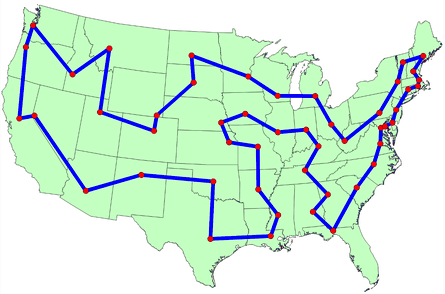
\includegraphics[width=0.9\textwidth]{graphics/48StatesTSP.png}

			\bigskip
			Algorithm \structure{MySuperTSPSolver}\\
			
\includegraphics[width=2cm]{graphics/hook.png}
		\end{center}
	\end{minipage}
	\qquad
	\frametitle{Motivation}
	\begin{minipage}{0.45\textwidth}
		\begin{center}
			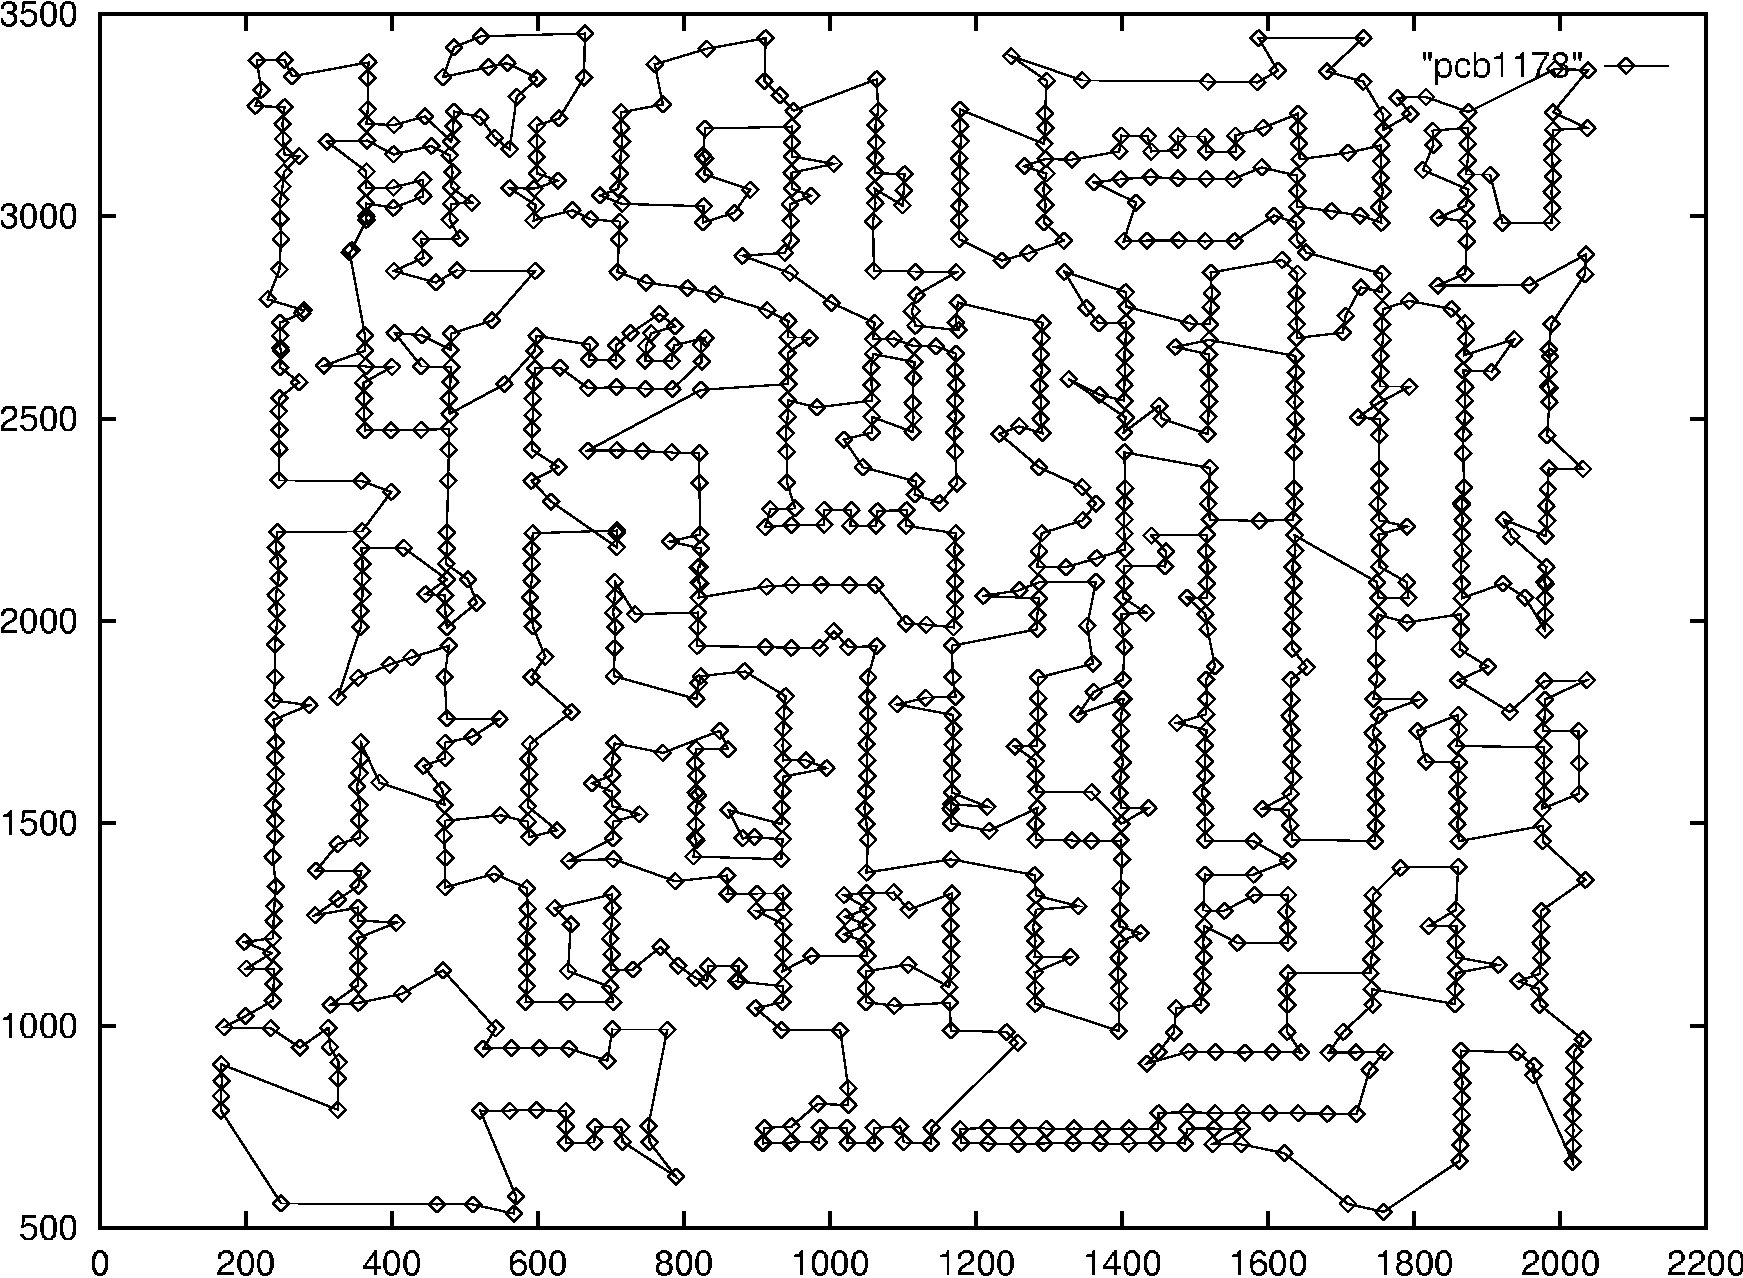
\includegraphics[width=0.9\textwidth]{graphics/TSPLeiter2opt.jpg}

			\bigskip
			\structure{MySuperTSPSolver} \alert{takes ``forever''}
			
\includegraphics[width=3cm]{graphics/question-mark.jpg}
		\end{center}
	\end{minipage}

\end{frame}

\begin{frame}{Motivation}

	\begin{center}
	\includegraphics<1>[width=0.4\textwidth]{graphics/hybrid-motivation.pdf}
	\includegraphics<2>[width=0.4\textwidth]{graphics/hybrid-motivation2.pdf}
	\end{center}

	\begin{itemize}
		\item 
		\structure{MySuperTSPSolver} does not scale well enough to (much) larger instances!
	
		\item \alert{Is different faster but cruder algorithm the only option?}
		\item<2> We aim at \important{\bf methods to improve the scalability} of MySuperTSPSolver,\\ (trading speed for quality).
	\end{itemize}
\end{frame}

\begin{frame}{Traditional/Naive Approaches}
	\begin{itemize}
	\item{\structure{Partition problem into smaller subproblems}\\
		solve them independently and combine solutions}\\
		\begin{center}
			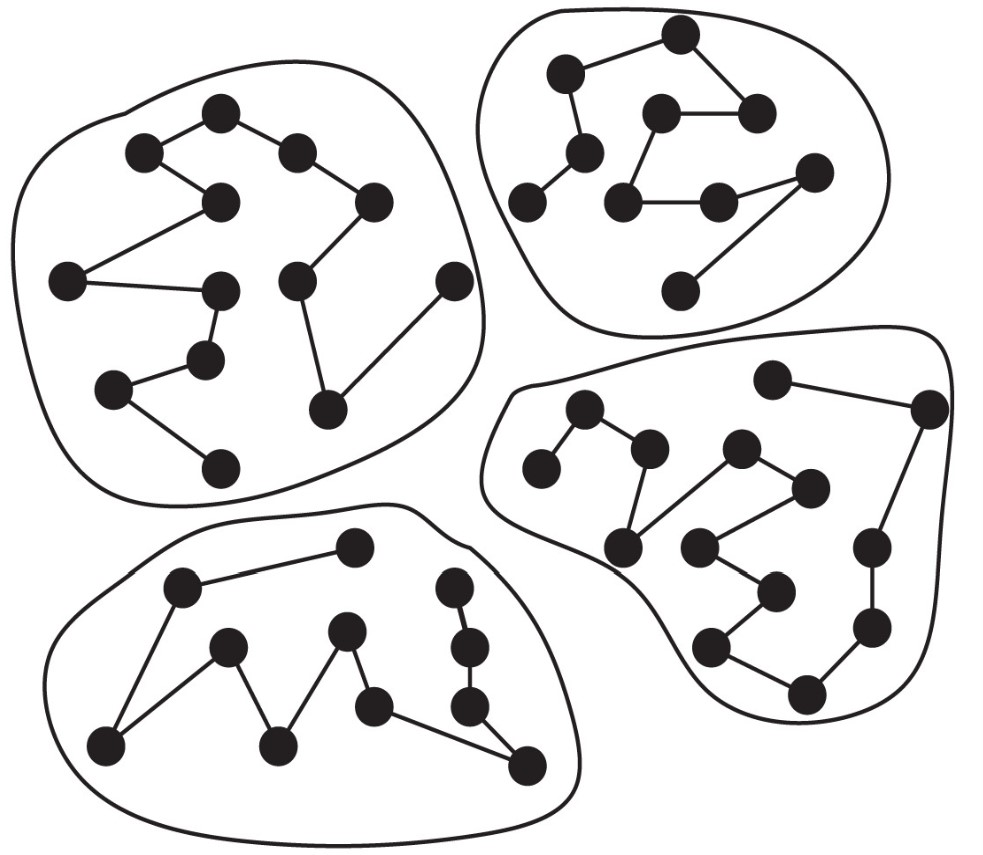
\includegraphics[width=0.22\textwidth]{graphics/partition.jpg}
		\end{center}
	\item<2>{\structure{Sparsifying the search space}}\\
		e.g., only consider $k$-nearest neighbor graph for TSP, VRP; \# edges: $O(n^2)\rightarrow O(n)$\\
		\begin{center}
			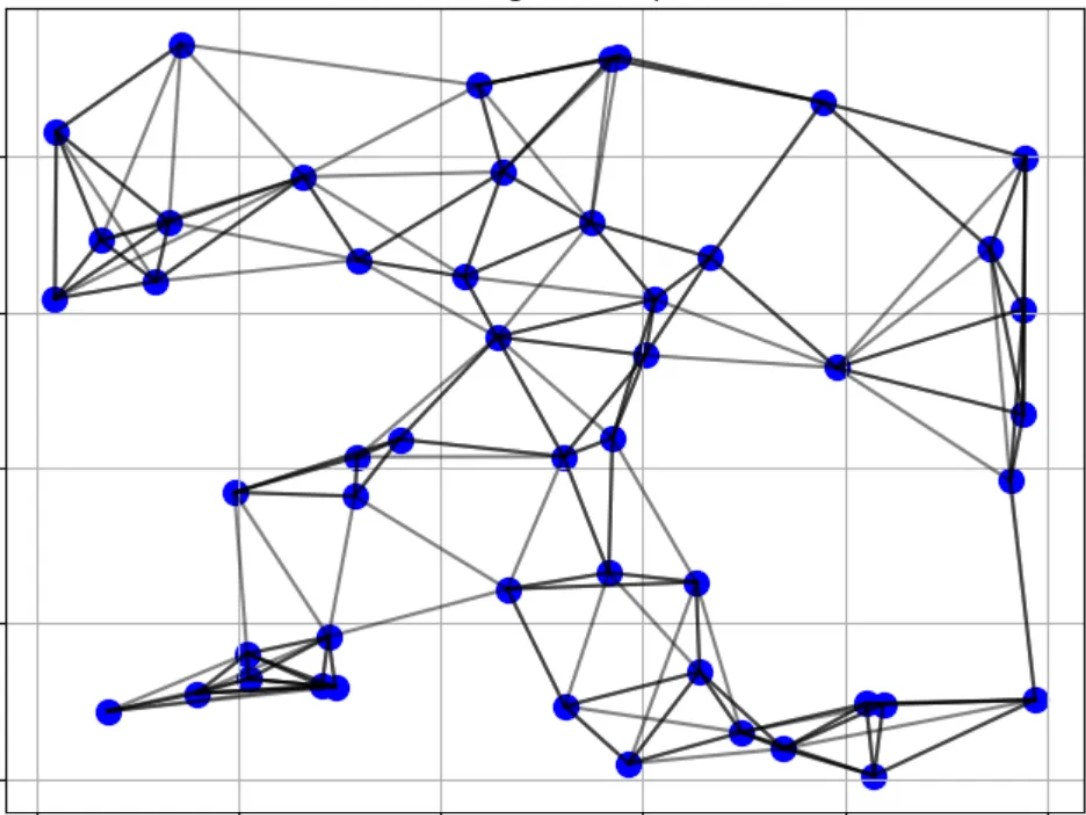
\includegraphics[width=0.28\textwidth]{graphics/kNN-graph.jpg}
		\end{center}
	\end{itemize}
\end{frame}

\begin{frame}{(Hybrid) Metaheuristic Approaches}
	\begin{itemize}
		\itemsep5ex
		\item \structure{Large Neighborhood Search (LNS)}\\
		\begin{itemize}
			\item Iteratively \important{destroy} parts of the solution by removing elements
			\item and \important{repair} it by solving the respective subproblem
			\item \alert{crucial:} choice of destroyed parts
		\end{itemize}
		\item \structure{Construct, Merge, Solve, and Adapt (CMSA)} \citep{blum-16b}
		\item \structure{POPMUSIC: Partial Optimization Metaheuristic Under Special Intensification Conditions} \citep{taillard-02}
		\item \ldots
	\end{itemize}
\end{frame}

\begin{frame}{Issues}
	While above strategies sometimes work well on academic problems,\\ they \alert{{\bf often fail} in more complex real-world scenarios}, e.g.,
	
	\bigskip
	\begin{itemize}
		\itemsep2ex
		\item because it is \alert{unclear which solution components are more or less promising}
		\item or \alert{more or less related to each other}. 
	\end{itemize}

	\vspace{1cm}
	\important{\bf Can we use machine learning for such aspects?}
	\begin{itemize}
		\item Focus here: offline, on representative training instances
	\end{itemize}
\end{frame}

% -----------------------------------------------------

\begin{frame}{A Multilevel Optimization Approach for
	Large Scale\\ Battery Exchange Station Location Planning}

\citep{jatschka-23}

\medskip
from a joint project with Honda Japan and Honda Research Institute Europe

\bigskip
\begin{center}
	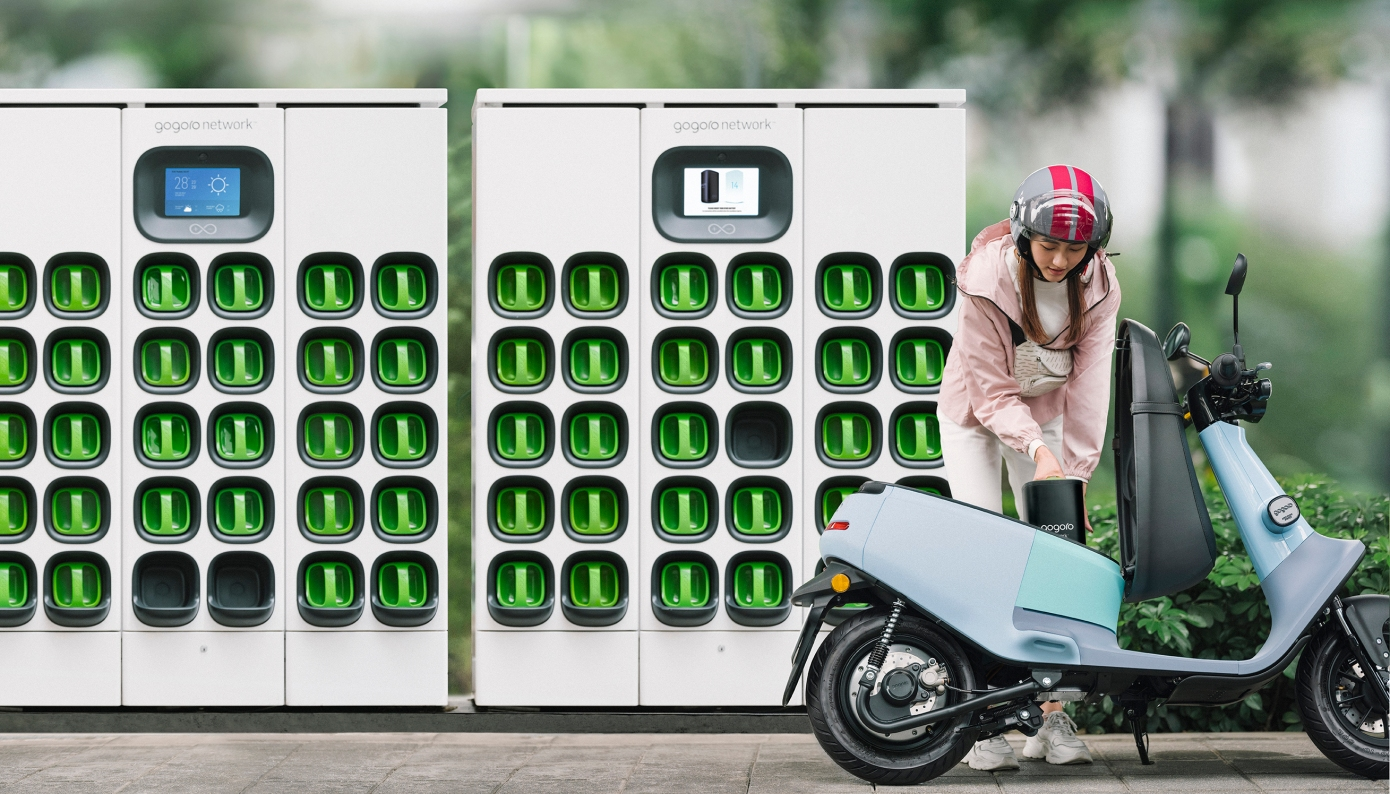
\includegraphics[width=0.6\textwidth]{graphics/Gogoro_Swapping_Station.jpg}\\
	{\small (c) Gogoro Inc.}
\end{center}
\end{frame}

\begin{frame}{Battery Exchange Station Location Planning (BEXLP)}
\begin{itemize}
\item \structure{Given:} 
	\begin{itemize}
		\item Potential locations for battery exchange stations
		\item Origin/Destination (O/D) pairs of expected trips \& frequency
	\end{itemize}
\item \structure{Goal:}
	\begin{itemize}
		\item Decide where to build stations with which capacities
		\item to maximize fulfilled demand while minimizing costs
	\end{itemize}
\end{itemize}

\begin{center}
	\includegraphics<1>[width=0.5\textwidth]{graphics/bex1.jpg}
	\includegraphics<2>[width=0.5\textwidth]{graphics/bex2.jpg}
	\includegraphics<3>[width=0.5\textwidth]{graphics/bex3.jpg}
	\includegraphics<4>[width=0.5\textwidth]{graphics/bex4.jpg}
	% 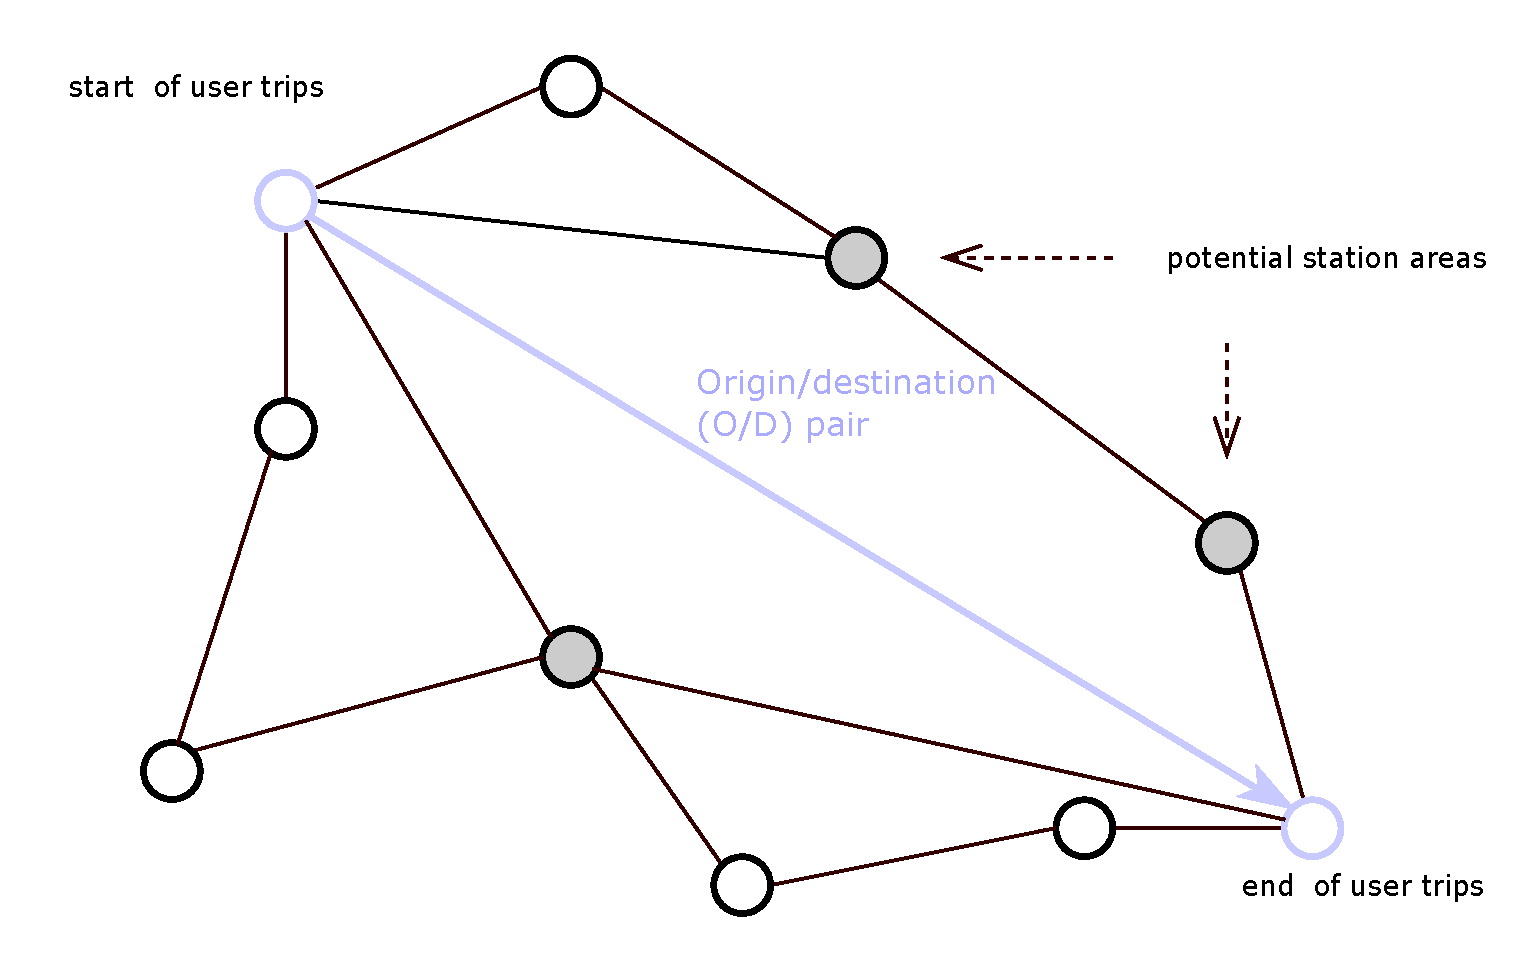
\includegraphics[width=0.6\textwidth]{graphics/graph_second.pdf}
	% \includegraphics<2>[width=0.6\textwidth]{graphics/graph_third.pdf}
\end{center}
\end{frame}

\begin{frame}{Fulfilled Demand of O/D Pairs}
\begin{itemize}
	\item Depends on \important{detour lengths} to close stations and their \important{capacities}
\end{itemize}
\begin{center}
	%\includegraphics<1>[width=0.6\textwidth]{graphics/graph_second.pdf}
	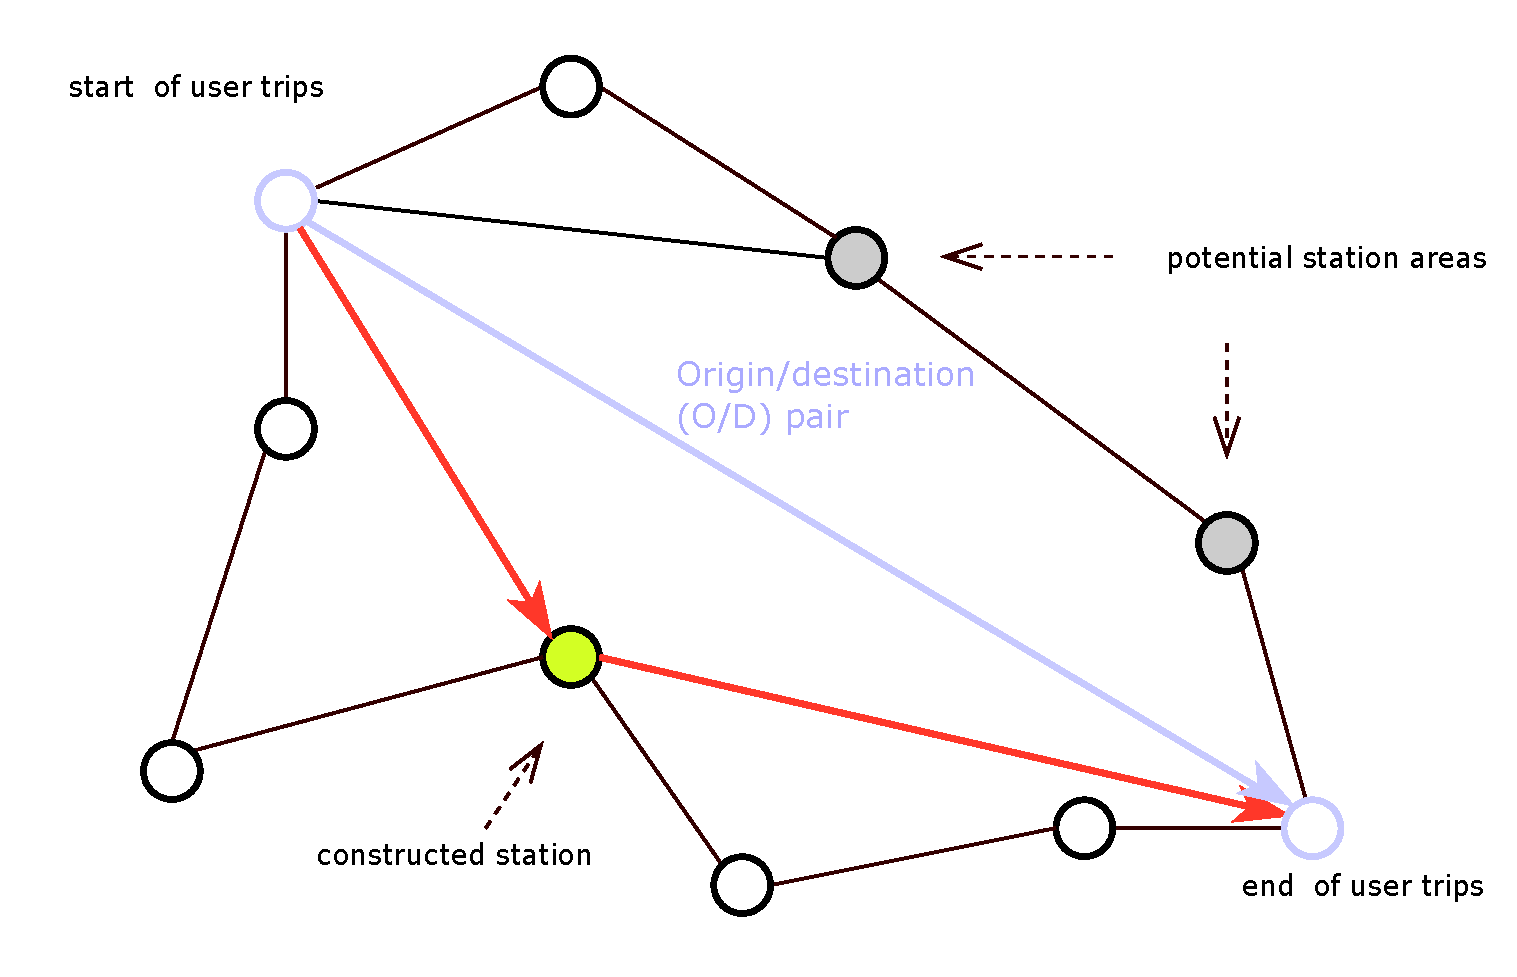
\includegraphics[width=0.6\textwidth]{graphics/graph_third.pdf}
	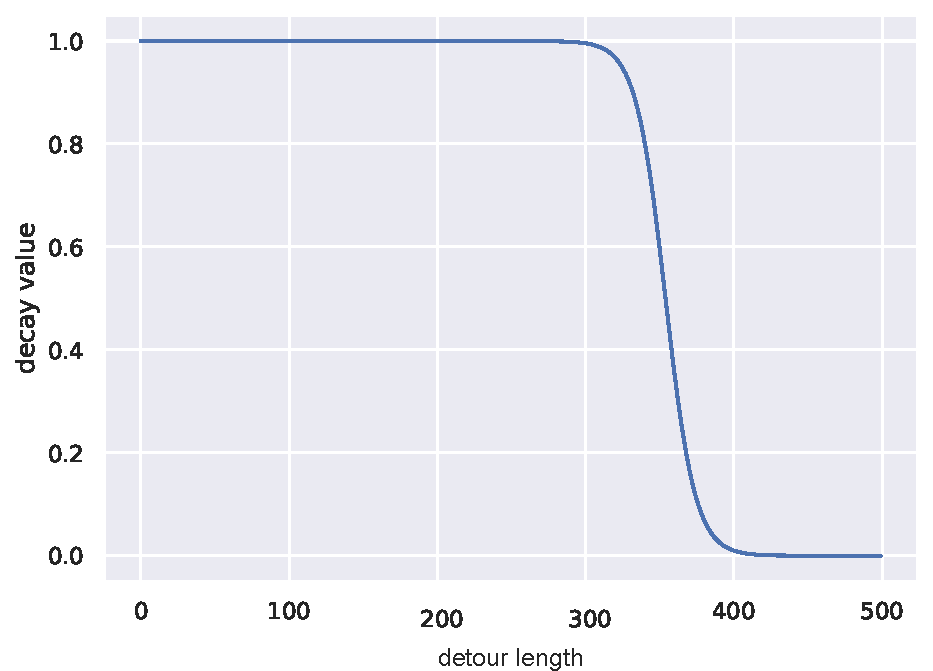
\includegraphics[width=0.35\textwidth]{graphics/decay.pdf}
\end{center}
\end{frame}

\begin{frame}{Solution Approaches}
	\begin{itemize}
		\itemsep3ex
		\item \important{Mixed Integer Linear Program (MILP)}:\\ works well for small instances with \alert{few hundred} nodes and O/D pairs
		\item \important{MILP-Based Large Neighborhood Search}:\\ can handle \alert{few thousand} nodes and O/D pairs
		\item \important{Multilevel Optimization}:\\ for instances with \alert{up to 10,000 nodes and 100,000 O/D pairs}
	\end{itemize}
\end{frame}


\begin{frame}{Multilevel Optimization (MLO) by \citet{walshaw-04}}

	\begin{enumerate}
		\item \important{\bf Coarsening}: Contract graph to smaller size
		\item Repeat (1) until threshold size is reached
		\item Solve problem on the coarsest graph
		\item \important{\bf Extend and refine} solution to the next level
		\item Repeat (4) until solution to original instance is obtained
			%\item \structure{Optional:} iteratively \important{\bf recoarsen} and extend+refine 
	\end{enumerate}

	\bigskip
	\begin{center}
		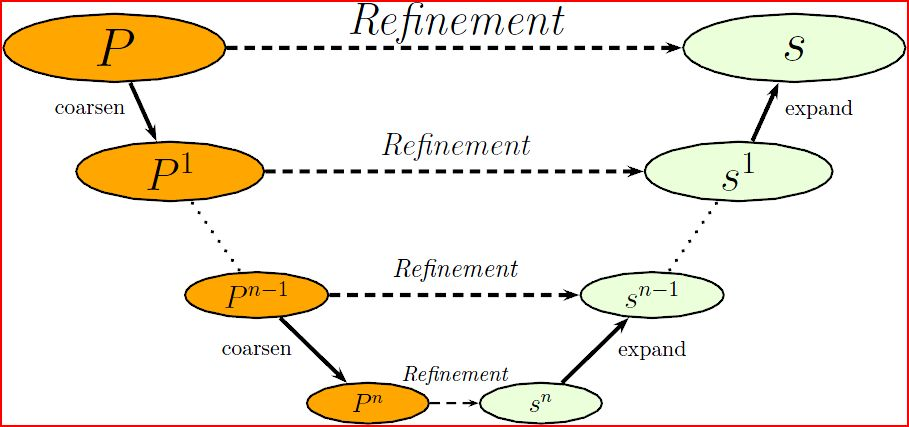
\includegraphics[width=0.6\textwidth]{graphics/multilevel.jpg}\\
		%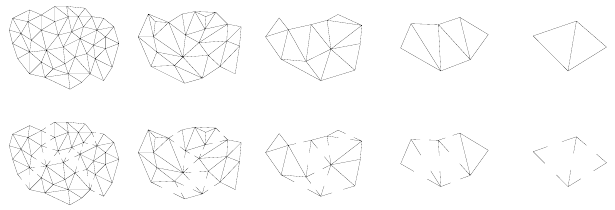
\includegraphics[width=0.6\textwidth]{graphics/mlr-gpp.png}
	\end{center}
\end{frame}

\begin{frame}{Multilevel Optimization (MLO) by \citet{walshaw-04}}
	\begin{center}
		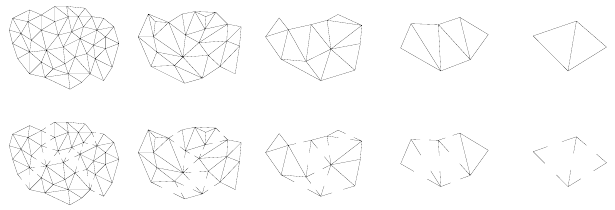
\includegraphics[width=0.9\textwidth]{graphics/mlr-gpp.png}\\
		{\small (for graph partitioning; from \citet{walshaw-04})}
	\end{center}

\important{Solution quality strongly depends on}
\begin{itemize}
	\item coarsening strategy
	\item extension and refinement strategies
\end{itemize}
\end{frame}

\begin{frame}{Multilevel Optimization for BEXLP}
\begin{center}
	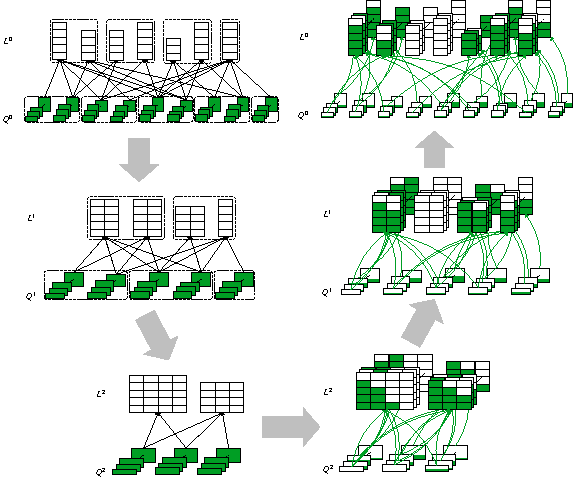
\includegraphics[scale=1.0]{graphics/MLR_example.pdf}
\end{center}
\end{frame}	

\begin{frame}{Multilevel Optimization for BEXLP}
\begin{itemize}
	\itemsep3ex
	\item Diverse clustering techniques considered
	\item MILP model used for extension/refinement
	\item Most challenging: What to take as \important{similarity measures} for
	\begin{itemize}
		\item O/D pairs to merge?
		\item for stations to merge?
	\end{itemize}
	\item Diverse similarity measures considered, ended up with Jaccard similarity
	\item In tests \important{$\approx$40--50\% better} than a reasonable construction heuristic
\end{itemize}
\end{frame}

\begin{frame}{Learning Multilevel Optimization for BEXLP}
	\citep{tomandl-24}

	\bigskip
	\begin{itemize}
		\itemsep2ex
		\item We \important{learned models to approximate the expected loss in solution quality} when
		\begin{itemize}
			\item merging two O/D pairs or 
			\item merging two stations, respectively
		\end{itemize} 
		\item Supervised learning with labels derived from
		\begin{itemize}
			\item merging pairs of nodes, solving, extension/refinement
			\item in comparison to solving original problem
		\end{itemize} 
		\item Models: multilayer perceptron with two hidden layers
		\item Diverse features derived from original nodes and merged nodes
		\item \important{Improvements of up to 1--5\% obtained}
		\item \important{Reasonable generalization to larger instances}
	\end{itemize}
\end{frame}

% -----------------------------------------------------

\begin{frame}
	\frametitle{The Electric Autonomous Dial-a-Ride Problem (EADARP)}

\citep{Bongiovanni:2019}
	
\structure{Given:} $n$ users with transportation requests from a pickup to a drop-off location,\\ a fleet of $m$ \important{electric autonomous} vehicles 

\medskip
\structure{Task:} Design $m$ vehicle routes serving all requests, s.t.\ the \important{total travel time and\\ the \textbf{excess ride times}} of all users are minimized and certain constraints are satisfied.
  
\begin{figure}
	\centering
	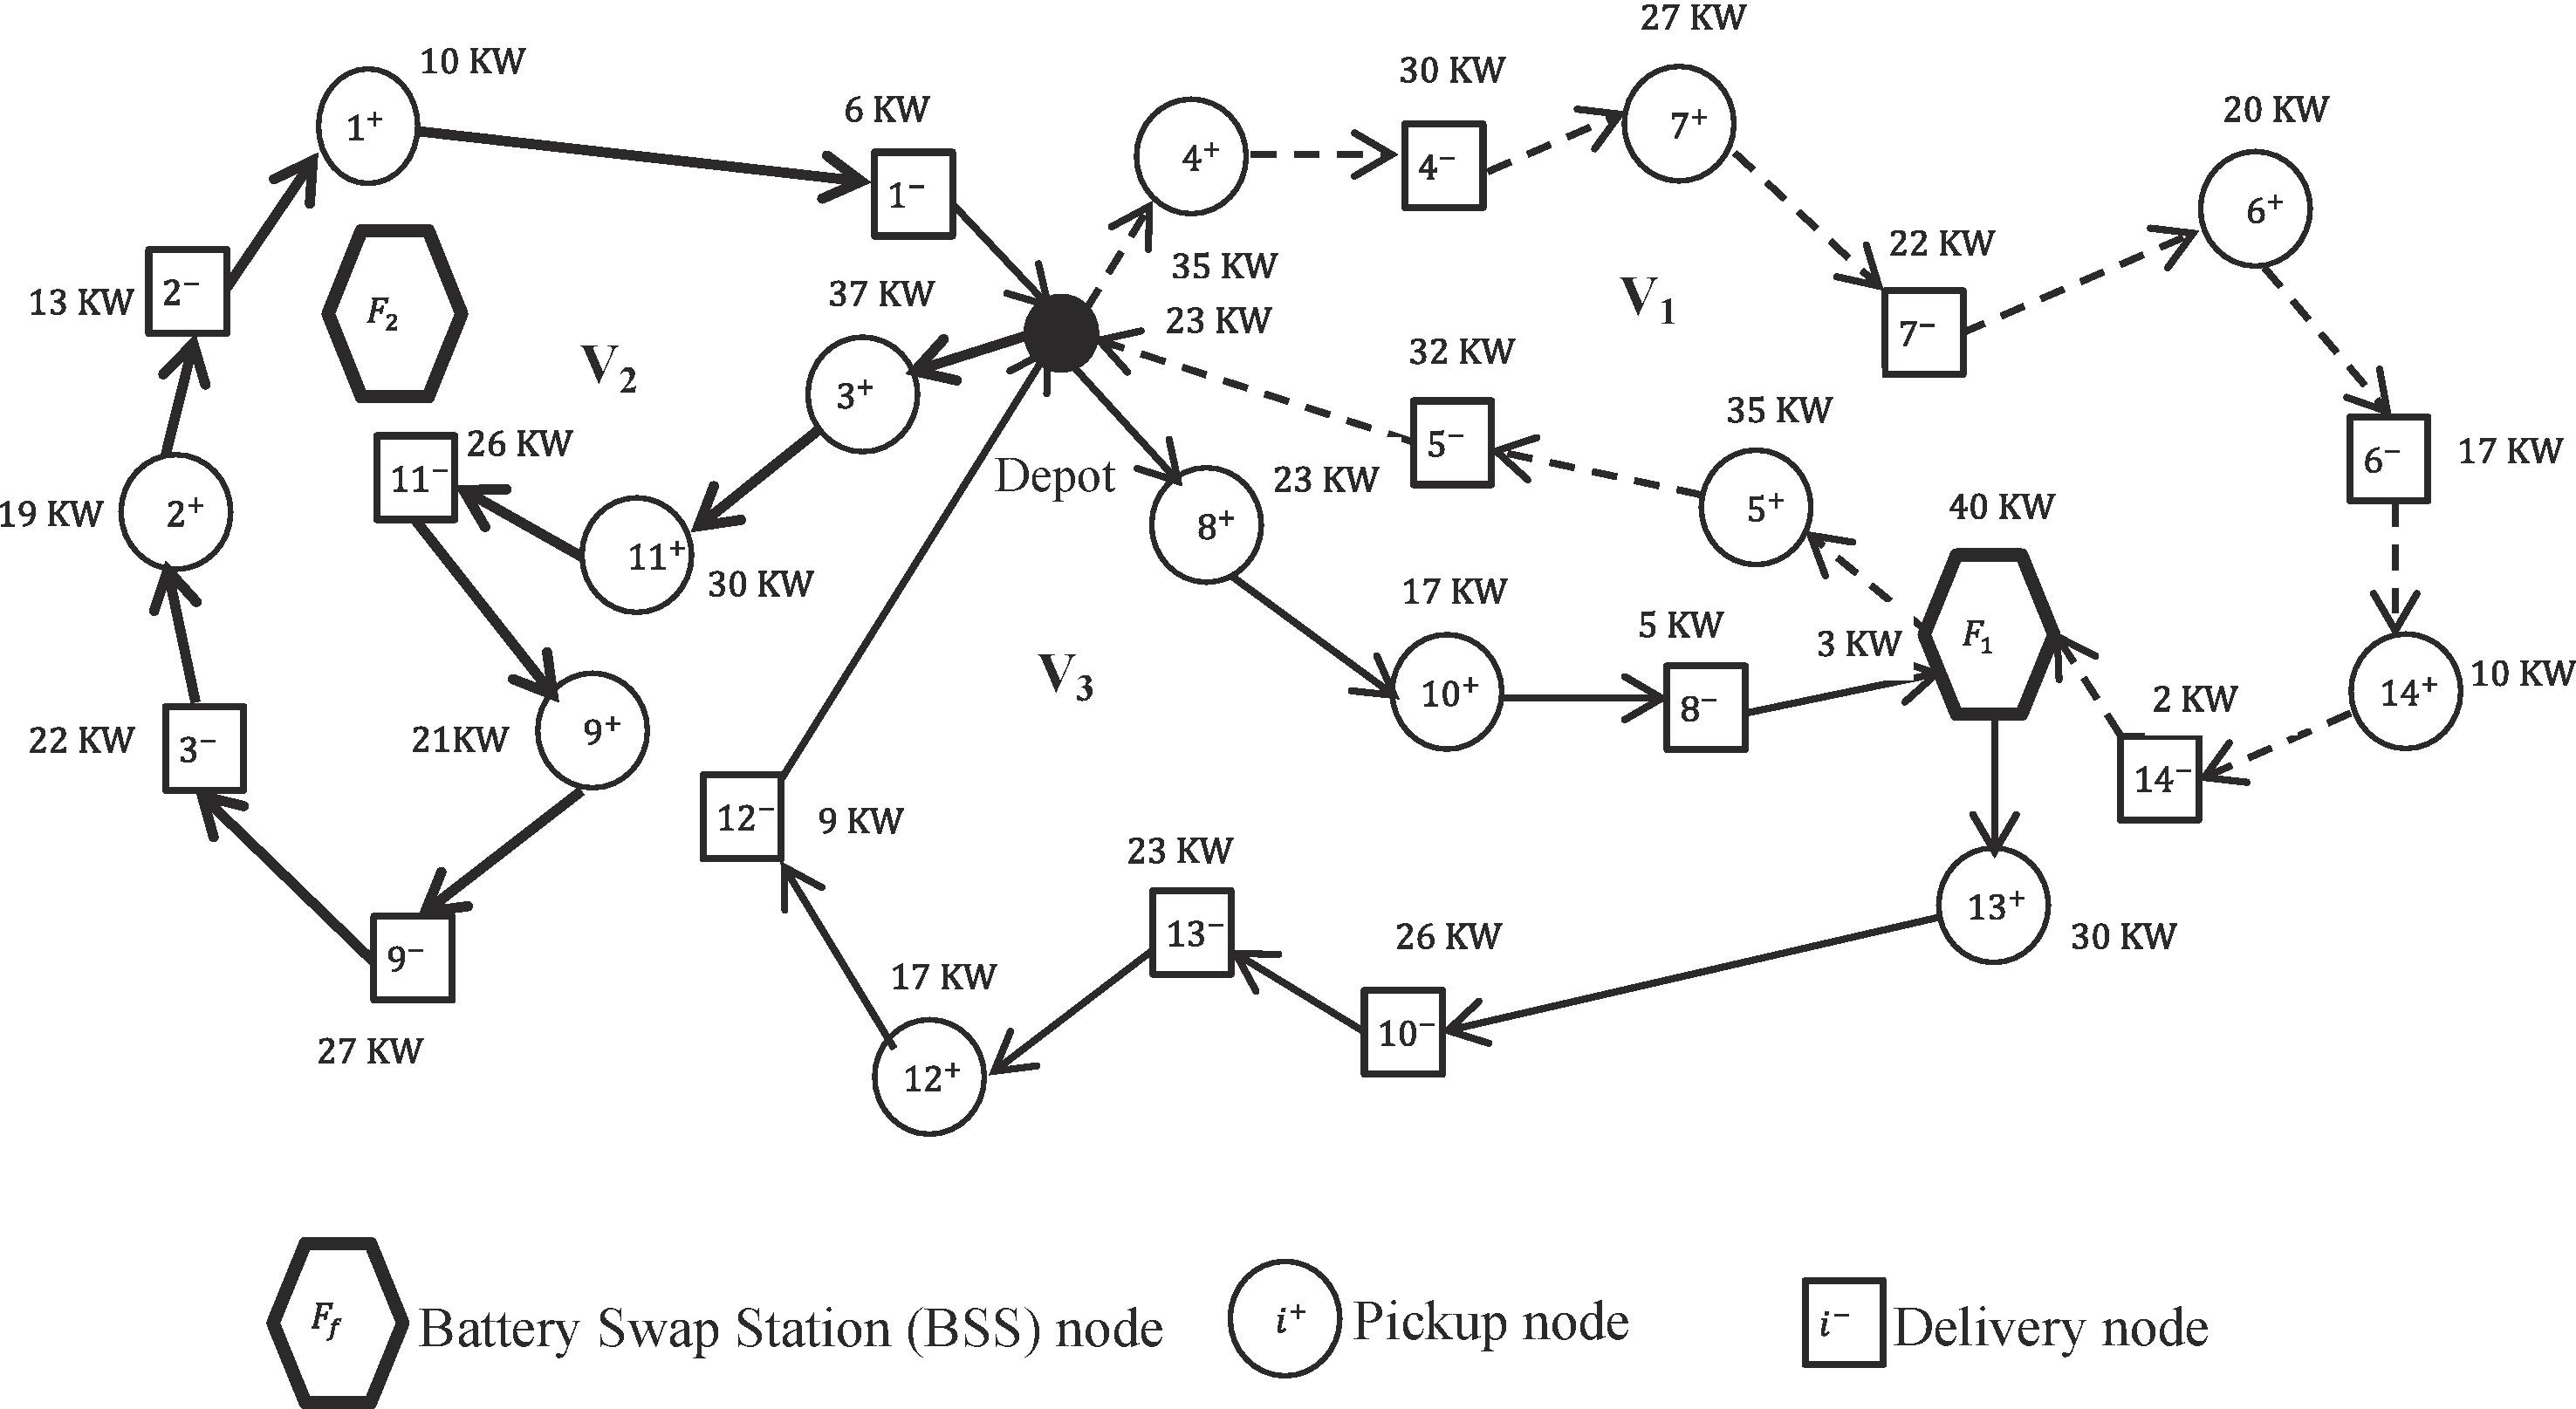
\includegraphics[scale=0.70]{graphics/darp-bss-example.jpg}
	%\caption{Example for E-DARP from \cite{Masmoudi:2018}.}
\end{figure}
	
\end{frame}

\begin{frame}
	\frametitle{Large Neighborhood Search for EADARP}

	(Bresich et al., 2024; GECCO 2024)

	\bigskip
	\begin{itemize}
		\itemsep3ex
		\item \structure{Key-feature:} an efficient algorithm to insert charging station visits into routes on-the-fly
		\item \important{Leading} for benchmark instances from literature with up to \important{100 users, 8 vehicles}
	\end{itemize}

	\bigskip
	\only<2>{However:}

	\bigskip
	\begin{itemize}
		\itemsep3ex
		\item<2> \citet{Limmer:2023}: Simpler and faster LNS also applicable to instances with\\
		\important{few hundred vehicles, several thousand users}
		\item<2> Our LNS only achieves \alert{few iterations within time-limit, gaps $~$10--30\%} 
		\item<2> \important{\bf How to scale up our LNS?}
	\end{itemize}

\end{frame}

\begin{frame}
	\frametitle{Sparsening Techniques for EADARP}

	\begin{itemize}
		\item \important{Sparsening to $k$-nearest neighbor graph:}\\
			\alert{Does not work well.} - Why? Each order has
		\begin{itemize}
			\item a pickup location
			\item a dropoff location
			\item a time window
		\end{itemize}
	\end{itemize}

	

\end{frame}

% -----------------------------------------------------


\begin{frame}{Denoising Diffusion Models (DDMs)}
\begin{itemize}
	\item State-of-the-art in many generative AI applications,\\
	in particular the creation of realistically-looking images

	\medskip
	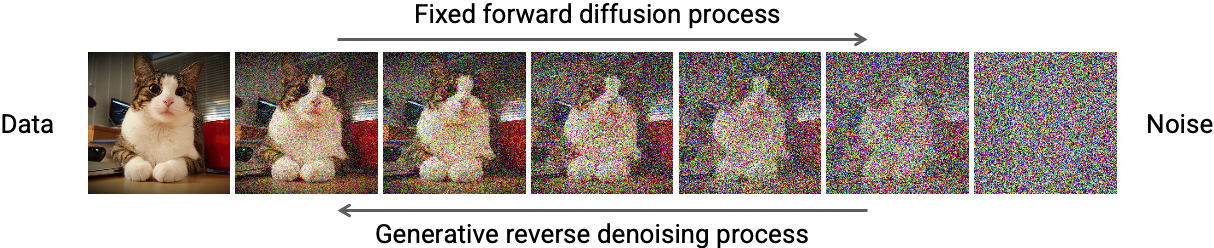
\includegraphics[width=0.9\textwidth]{graphics/diffusion.png}

	\bigskip
	\item \structure{Training}
	\begin{itemize}
		\item Gaussian noise step-wise added to original images
		\item Neural network trained to predict noise added in each step
	\end{itemize}
	\item \structure{Inference}
	\begin{itemize}
		\item Starts from pure random noise
		\item Stepwise remove noise via neural network
	\end{itemize}
	\item DDMs can be conditioned on additional input
	\item \important{Concept can also be applied to graph neural networks!}
\end{itemize}
\end{frame}

\begin{frame}
	\frametitle{DIFUSCO: Graph-Based Diffusion Solver for Combinatorial Opt.} 
	
	\citep{sun-23}

	\bigskip
	\begin{itemize}
		\itemsep1ex
		\item TSP and maximum independent set problem considered
		\item utilizes an anisotropic \important{graph neural network} with edge gating
		\item \important{discrete diffusion} based on Bernoulli noise
		\item trained on many small instances + (close to) optimal solutions
		\item used to create \important{diverse heatmaps} 
		\item greedy heuristics and MCTS used as decoder
	\end{itemize}

	\bigskip
	\only<1>{\centering 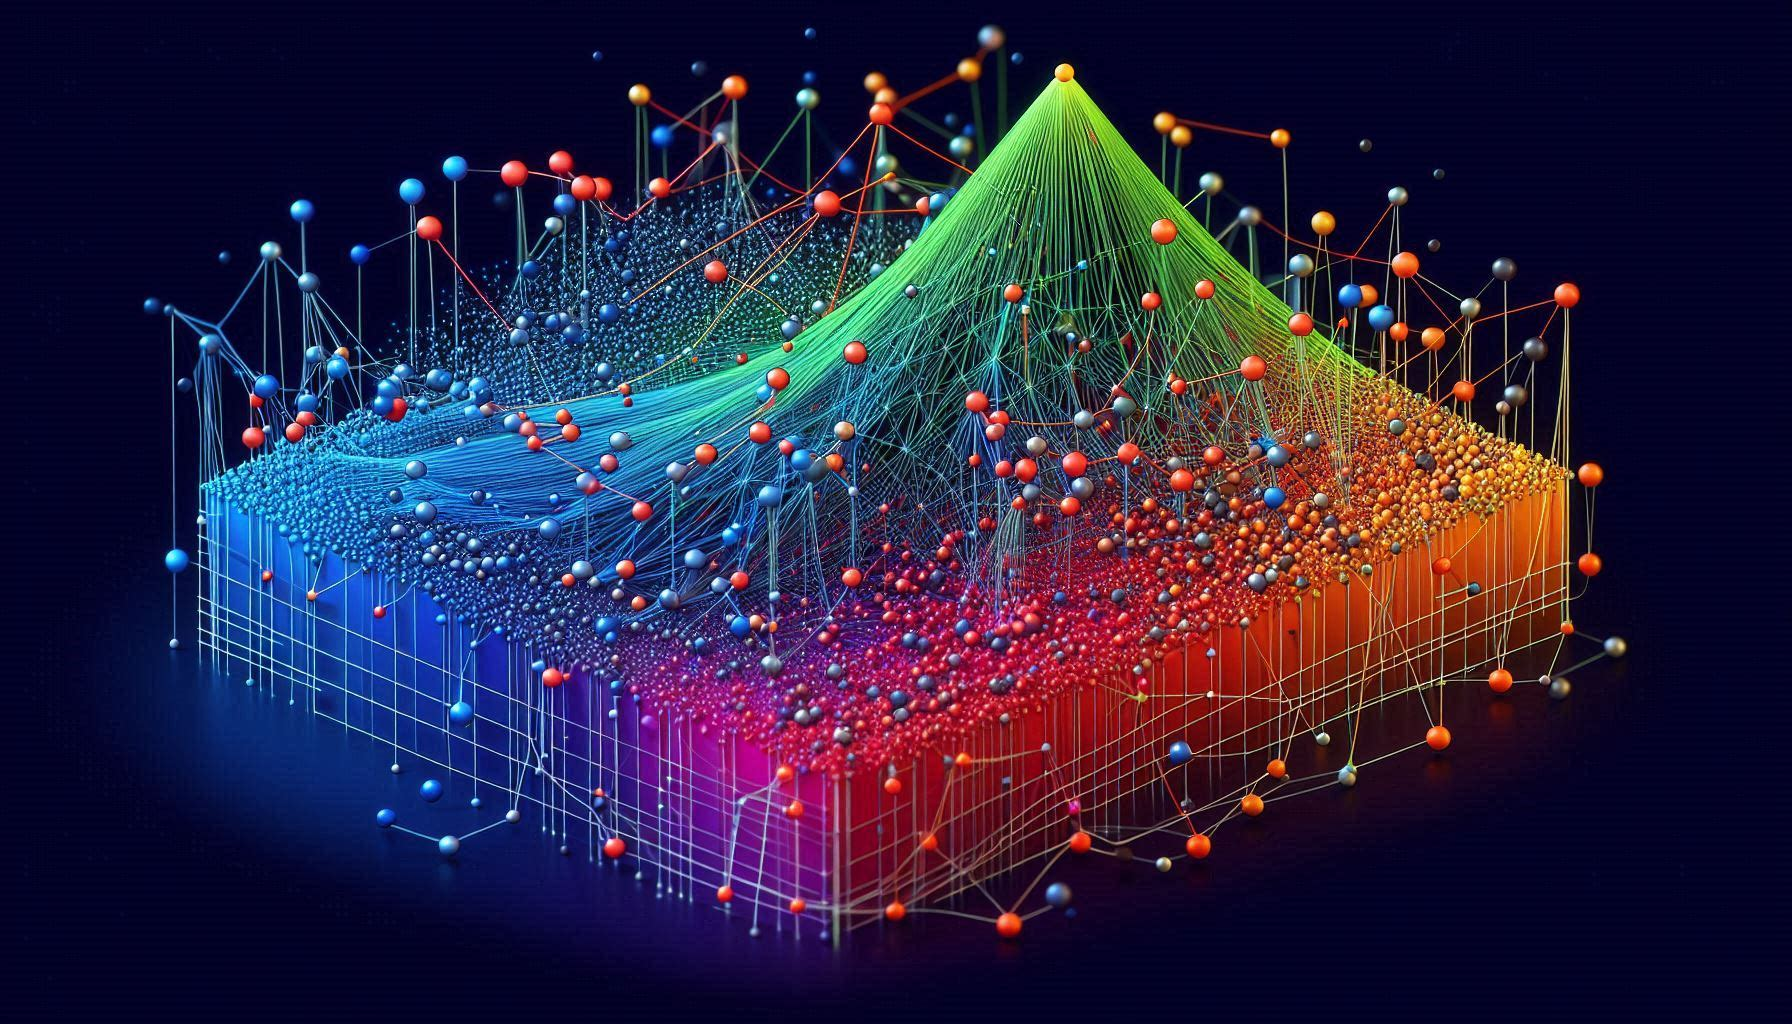
\includegraphics[width=0.4\textwidth]{graphics/graphdiff.png}}
	\only<2>{\begin{itemize}
		\item<2> \structure{Advantages}
		\begin{itemize}
			\item \alert{outperforms earlier approaches} by a large margin in their tests
			\item \alert{faster} than autoregressive models
			\item \alert{better scaling behavior} to larger instances
			\item \alert{multi-modality of solution space is considered}
		\end{itemize}
	\end{itemize}}
\end{frame}

\begin{frame}
	\frametitle{DIFUSCO: Graph-Based Diffusion Solver for Combinatorial Opt.}

	\begin{center}
		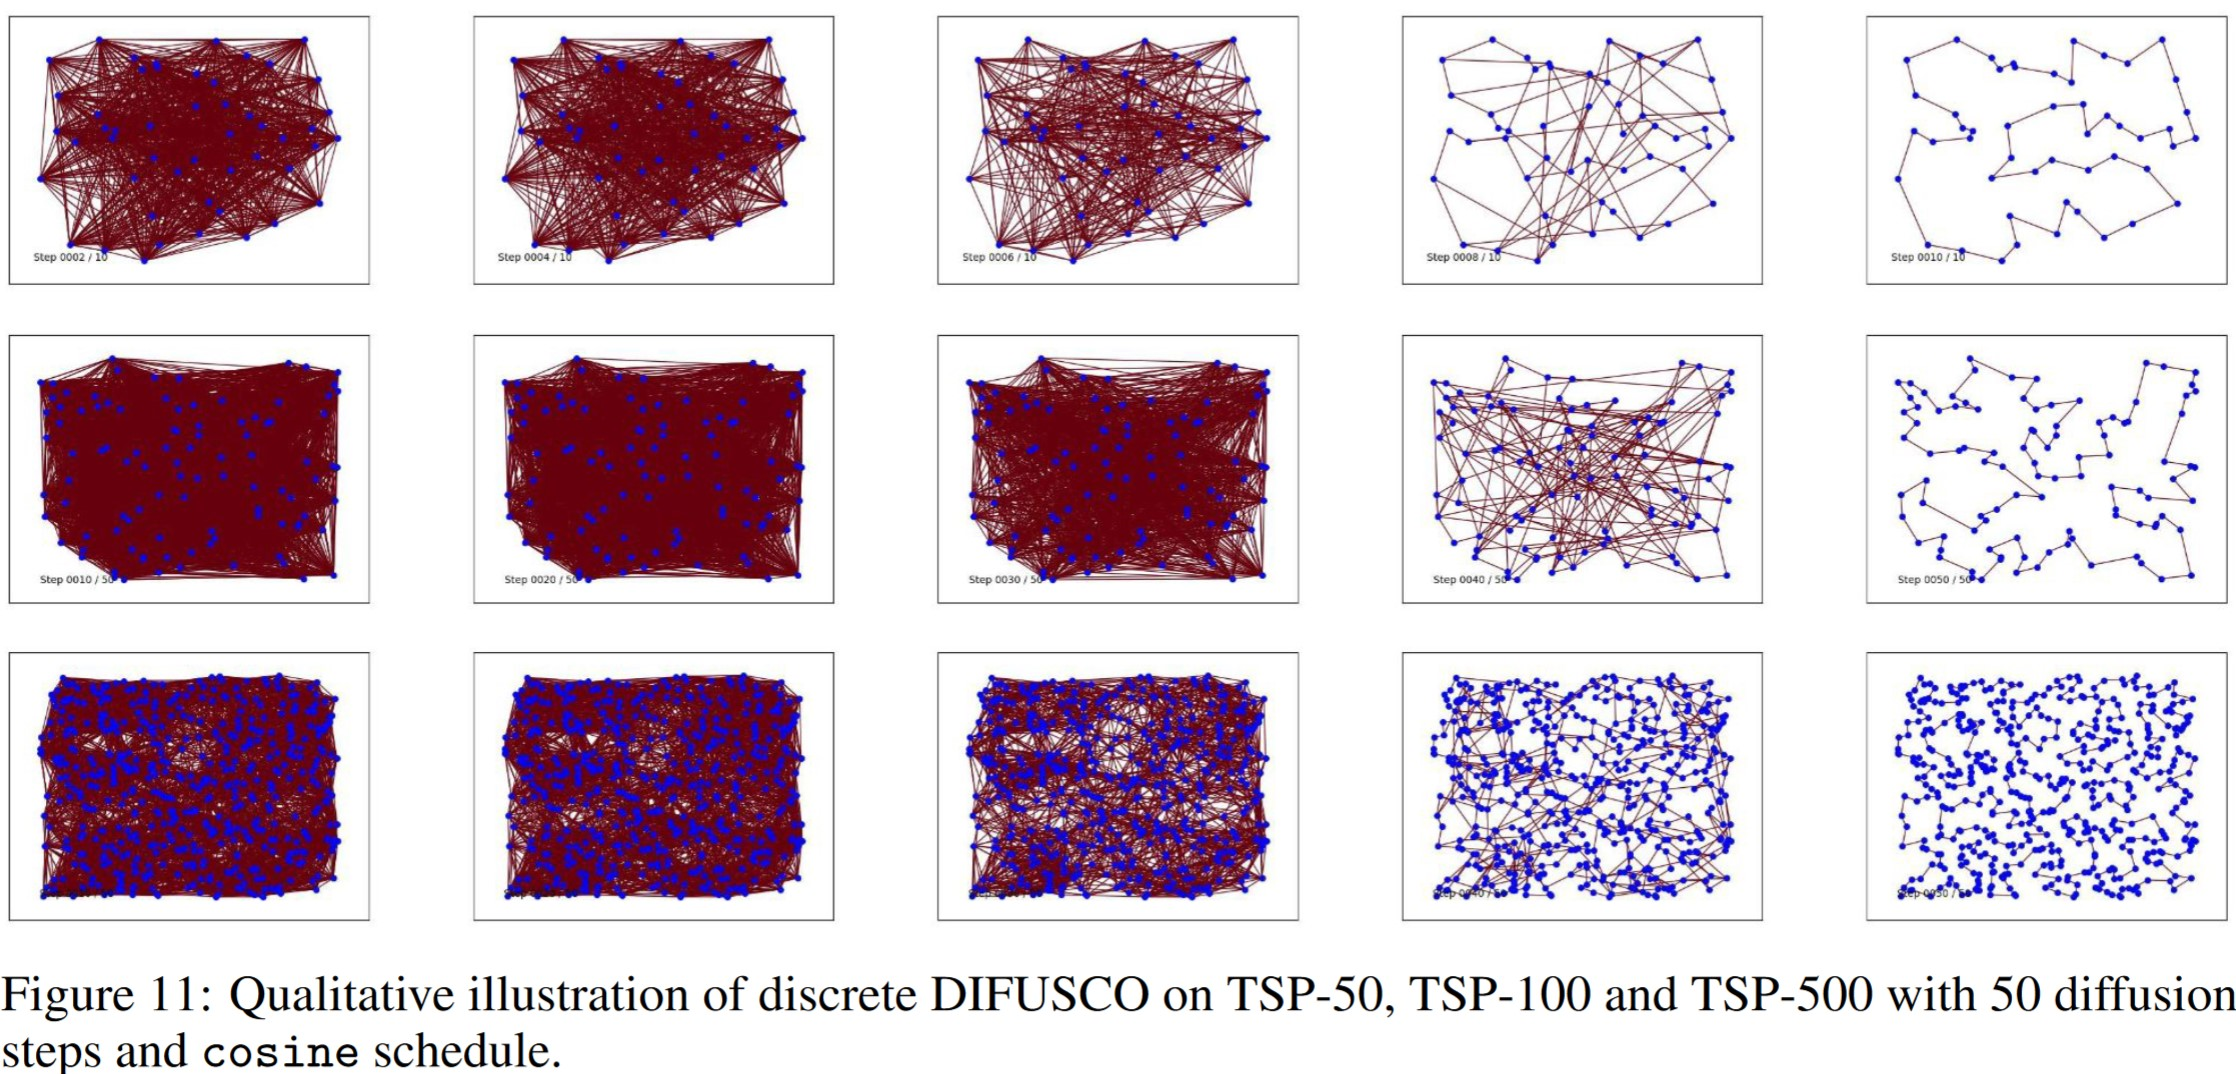
\includegraphics[width=\textwidth]{graphics/difusco1.jpg}
		(from \citet{sun-23})
	\end{center}
\end{frame}

\begin{frame}
	\frametitle{DIFUSCO: Graph-Based Diffusion Solver for Combinatorial Opt.}

	\begin{center}
		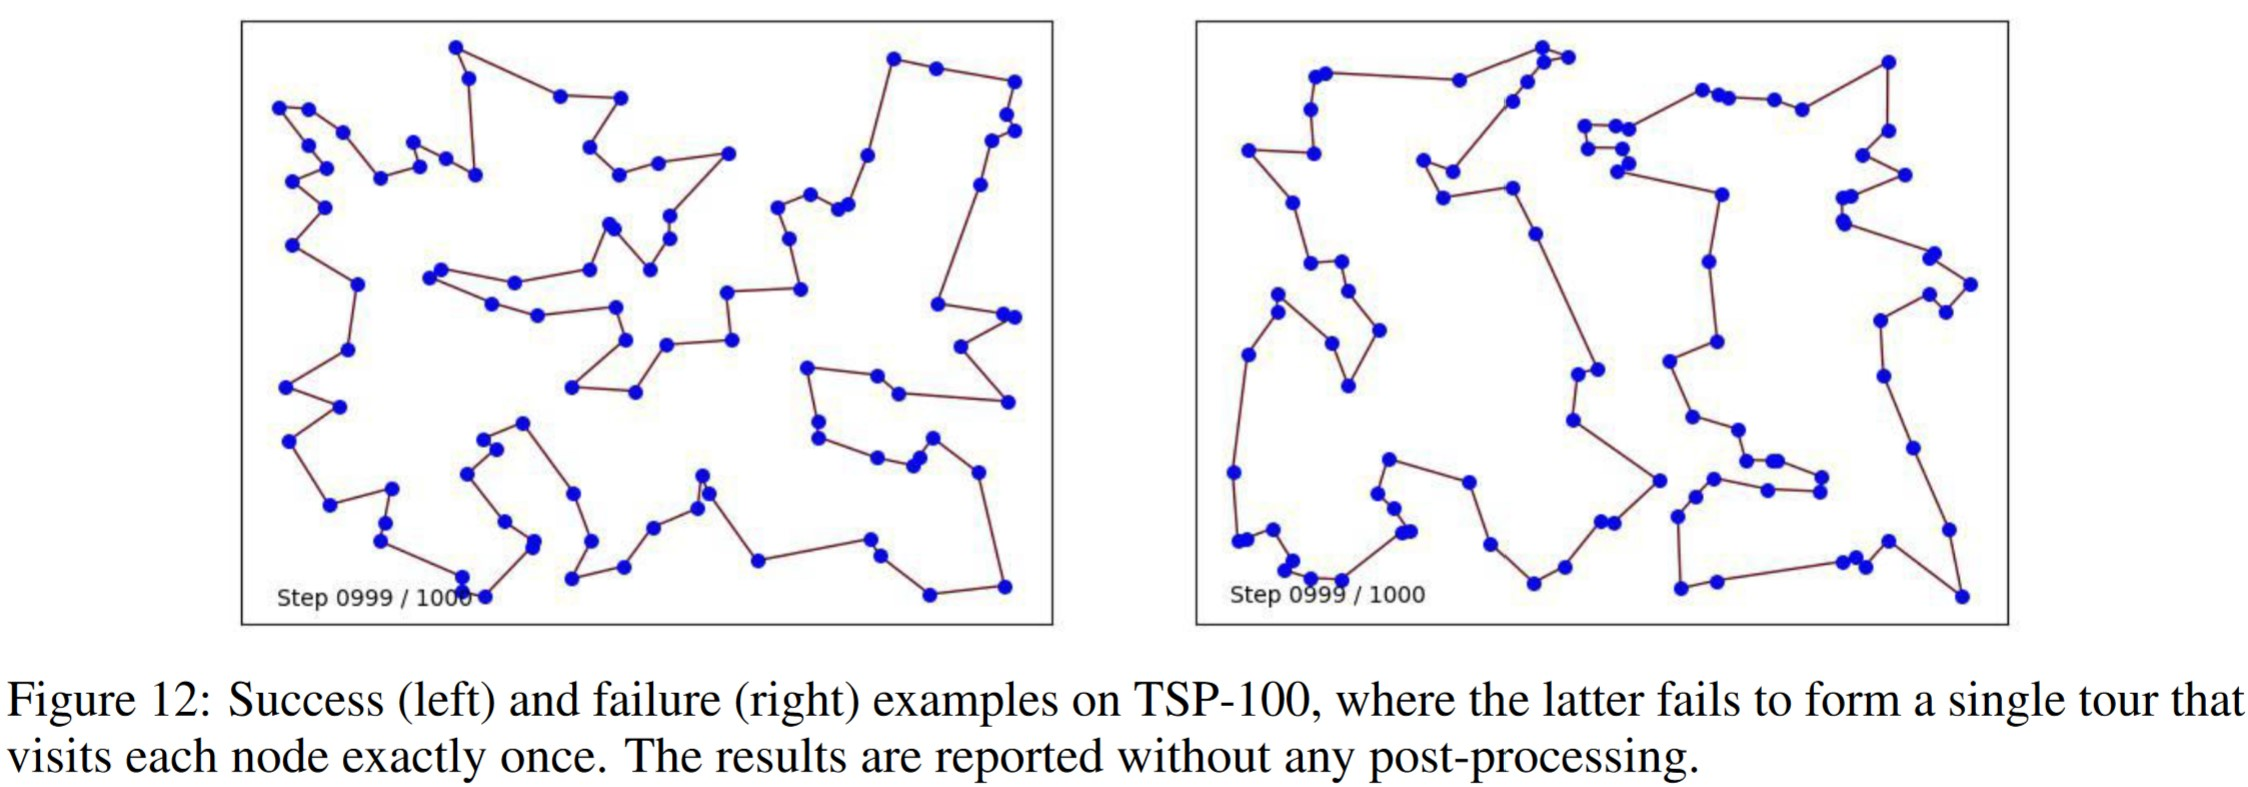
\includegraphics[width=\textwidth]{graphics/difusco2.jpg}
		(from \citet{sun-23})
	\end{center}
\end{frame}


\begin{frame}
	\frametitle{Own Ongoing Work}
	We are currently investigating \important{DDM \& GNN-based approaches for EADARP} 
		\begin{itemize}
			\item to determine destroy sets in LNS
			\item to restrict candidate routes for order insertions
			\item to restrict candidate positions for order insertions
			\item to dynamically decompose problem instances
		\end{itemize}
	
	\bigskip
	Related DDM \& GNN-based methods are also investigated on
	\begin{itemize}
		\item graph burning problem
		\item $\alpha$-domination problem
		\item maximum influence problems in graphs
	\end{itemize}
	
	\bigskip
	\important{\bf Early results promising!}
\end{frame}

\begin{frame}{Conclusions}
	\begin{itemize}
		\itemsep3ex
		\item Manifold strategies to improve scaling of solving approaches for COP
		\item Sometimes basic strategies work already well, sometimes much harder
		\item End-to-end learning approaches will not soon replace classical CO techniques in general
		\item ML can help substantially to
			\begin{itemize}
				\item sparsify search space
				\item find better problem decompositions
				\item better focus search operators 
			\end{itemize} 
		\item Graph \& DDM-based approaches currently particularly promising?
	\end{itemize}
\end{frame}

	% \frametitle{Ideas to Utilize DDMs in Population-Based MHs}
	% \begin{itemize}
	% 	\item for creating diverse initial solutions
	% 	\item for a kind of intelligent recombination(?)
	% \end{itemize}


% ### Bibliography ################################################################################

\begin{frame}[allowframebreaks]
	\frametitle{References}
	%\fontsize{6pt}{7.2}\selectfont
	\small
	\bibliography{lit}
\end{frame}

\end{document}

